\documentclass[UTF8,12pt,a4paper]{ctexart}

\usepackage[a4paper,margin=2.2cm]{geometry}
\usepackage{amsmath}
\usepackage{amssymb}
\usepackage{booktabs}
\usepackage{graphicx}
\usepackage{float}
\usepackage[numbers,sort&compress]{natbib}
\usepackage[hidelinks]{hyperref}
\usepackage{setspace}

\setstretch{1.3}
\emergencystretch=2em
\newcommand{\cmark}{\checkmark}
\newcommand{\xmark}{--}

\title{UAV-TAlign-12K：面向跨视场无人机\\红外-可见光对齐的场景级可靠性基准}
\author{匿名作者}
\date{中文审阅稿，与英文投稿稿同步}

\begin{document}

\maketitle

\begin{abstract}
跨视场红外-可见光对齐是无人机巡检、夜间感知与多模态场景理解中的核心能力。
本文提出 UAV-TAlign-12K：一个基准规模的数据集，包含从 15 个工业与自然场景采集的
6,039 对同步 RGB-红外图像，并提供经过完整性检查的 6,037 对正式评测划分。
该基准从三个互补层级组织评测：成对单应性证据、场景级共识，以及可靠性--覆盖率运行分析。
七种代表性方法涵盖经典关键点流程、红外-可见光专用匹配方法，以及现代稠密或学习型匹配器。
成对证据在整体上具有很高可用性：RIFT2、RoMa 与 raw MINIMA 在全部 6,037 对图像上均能
生成单应性，而 LoFTR 与 XoFTR 的可用率均超过 99\%。在此基础上，UAV-TAlign 结合渐进式
证据调度、几何校准帧加权、鲁棒场景共识与跨模态质量验证。该框架为全部 15 个场景估计变换，
并在规范运行点识别出 9 个高置信对齐产品，覆盖 74.4\% 的评测图像对。五折留帧分析得到
1.39 像素的场景共识漂移中位数；受控平移、旋转与尺度扰动则使联合质量信号单调下降。
UAV-TAlign-12K 为基准规模、置信度感知的无人机红外-可见光对齐研究建立了可复现基础。
\end{abstract}

\noindent\textbf{主要要点}
\begin{itemize}
\item UAV-TAlign-12K 提供 6,039 对同步跨视场无人机 RGB-红外图像。
\item 七种基线表明，成对单应性证据已具有广泛可用性。
\item UAV-TAlign 生成 15 个场景变换，并识别出 9 个高置信场景产品。
\item 重采样和受控扰动验证了所提出的运行协议。
\end{itemize}

\noindent\textbf{关键词：} 红外-可见光数据集；无人机影像；多模态配准；对齐基准；场景级可靠性

% !TEX root = ../paper_zh.tex

\section{引言}

红外-可见光对齐是无人机巡检、夜间监测与多模态热感知中的基础能力。可见光影像提供语义与
结构细节，而红外影像可在光照变化、烟雾、薄霾和低照度条件下保留互补的目标信息。两种模态
的结合已经支撑了多光谱检测、跟踪以及复杂运行环境中的航空感知
\cite{hwang2015kaist,flir2018thermal,jia2021llvip,liu2022tardal,sun2022dronevehicle,zhang2022vtuav,li2022lasher,jiang2023antiuav}。
因此，要将两路数据视为一个统一的传感系统，而非彼此独立的观测，就必须准确恢复跨传感器几何关系。

无人机采集引出了一个具有自身特点的对齐问题。跨视场光学系统、不一致的传感器分辨率、变化的
视角以及变焦会使同一场景在可见光和红外通道中呈现不同几何形态。热成像渲染方式以及昼夜外观
变化还会进一步改变局部纹理和对比度。因此，一段飞行序列会提供异质的几何证据：不同图像对在
空间支撑、单应性稳定性以及跨模态一致性方面可能存在显著差异。有效的对齐方法需要将这些证据
整合为可服务于下游感知任务的场景变换。

现代对应关系估计方法已经显著提高了成对证据的可用性。LoFTR、LightGlue、DKM、RoMa、XoFTR
和 MINIMA 等 Transformer、稠密与多模态匹配器，能够在越来越困难的外观变化下恢复对应关系
\cite{sarlin2020superglue,sun2021loftr,chen2022aspanformer,lindenberger2023lightglue,edstedt2023dkm,edstedt2024roma,tuzcuoglu2024xoftr,ren2025minima}。
近期无人机对齐基准也引入了合成变换监督与直接几何评测 \cite{gao2025uavmatch}。这些进展建立了
强大的成对匹配基础，同时也提出了更高层次的基准问题：应如何在真实无人机场景尺度上整合并评估
质量不一的逐帧估计？

本文通过 UAV-TAlign-12K 回答这一问题。该基准包含来自 15 个工业与自然场景的 6,039 对真实采集
跨视场无人机红外-可见光图像。正式评测划分包含 6,037 对经过完整性检查的图像，覆盖白天、夜间
与低照度采集，灰度与伪彩红外渲染，以及广角、变焦和常规无人机视图。该基准定义了三个互补的
评测轨道：成对评测衡量单应性证据可用性；场景级评测衡量多帧共识产品；可靠性--覆盖率曲线刻画
可选择的运行区间。这个层级结构将对应关系生成与无人机感知系统所需的场景产品联系起来。

UAV-TAlign 是该基准的参考框架。它构建在强成对匹配器之上，并结合渐进式证据调度、几何校准
帧加权、鲁棒场景共识和跨模态质量验证。在正式评测划分上，红外专用方法和现代匹配器均能提供
高可用性的成对单应性。UAV-TAlign 将这些证据转化为全部 15 个场景的变换，并在规范运行点识别
出 9 个高置信场景产品，覆盖 74.4\% 的评测图像对。受控扰动和留帧重采样分别从几何敏感性与
证据稳定性两个方面支撑了所得运行曲线。

本文的主要贡献包括：
\begin{itemize}
\item 提出 UAV-TAlign-12K，一个包含 15 个多样化场景、6,039 对同步图像及 6,037 对完整性检查
评测划分的真实跨视场无人机红外-可见光基准。
\item 构建覆盖成对单应性证据、场景级共识与可靠性--覆盖率分析的多层评测协议，并通过条件感知
诊断、重采样稳定性和受控扰动对其进行验证。
\item 提出 UAV-TAlign 参考框架，通过渐进式证据调度、鲁棒共识和跨模态质量验证，将强成对证据
转化为高置信场景产品。
\end{itemize}

% !TEX root = ../paper_zh.tex

\section{相关工作}

\subsection{跨模态对应关系与几何估计}

经典配准流程通常结合局部特征提取、描述子匹配与鲁棒模型估计。尺度空间、二进制以及非线性扩散
特征为多种成像条件提供了高效的几何参考
\cite{lowe2004sift,bay2008surf,rublee2011orb,leutenegger2011brisk,alcantarilla2012kaze,alcantarilla2013akaze}。
RANSAC 及其面向精度改进的后续方法，仍是将含噪对应关系转化为几何模型的核心技术
\cite{fischler1981ransac,hartley2004multiple,barath2019magsac,barath2020magsacpp}。
针对红外-可见光影像，RIFT 等辐射变化不敏感方法提高了描述子在模态特有外观变化下的重复性
\cite{li2020rift}。这些方法为区分“对应关系质量”和“后续场景聚合”提供了可解释的基础。

学习型对应关系方法同时扩展了成对证据的鲁棒性和空间密度。早期可训练检测器与描述子建立了
数据驱动的局部表示
\cite{detone2018superpoint,ono2018lfnet,dusmanu2019d2net,revaud2019r2d2,tyszkiewicz2020disk,germain2020s2dnet,mishchuk2017hardnet,tian2017l2net,tian2019sosnet}。
随后，图推理、Transformer 与稠密形变预测使方法能够直接处理低纹理、重复结构和大幅外观变化
\cite{sarlin2020superglue,rocco2018ncnet,zhou2021patch2pix,jiang2021cotr,sun2021loftr,chen2022aspanformer,lindenberger2023lightglue,edstedt2023dkm,edstedt2024roma,wang2024efficientloftr,jiang2024omniglue}。
XoFTR 与 MINIMA 进一步面向可见光-热红外或更广泛的多模态对应关系
\cite{tuzcuoglu2024xoftr,ren2025minima}。UAV-TAlign 在这些进展之上，将成对匹配器视为场景级几何
流程中的证据生成器。

\subsection{红外-可见光对齐}

红外-可见光配准涵盖基于特征的匹配、直接优化与学习型对齐。辐射不敏感描述子用于处理非线性
跨模态外观差异，而学习型方法则从训练数据中估计成对变换或稠密形变
\cite{li2020rift,chang2017clkn,nie2021udis}。无人机双传感器影像还叠加了跨分辨率光学、视点位移、
热成像渲染变化和光照变化。这些条件推动了专用成对方法和无人机数据资源的发展。

UAVMatch 为可训练无人机对齐提供合成变换监督和受控几何指标 \cite{gao2025uavmatch}。
ATR-UMMIM 提供 7,969 组真实无人机可见光--红外--已配准可见光三元组，并包含条件属性和半自动
像素级参考 \cite{bin2025atrummim}。UAV-TIRVis 提供 80 对人工配准的航空热红外-可见光图像，用于
直接图像域评测 \cite{vasile2025uavtirvis}。UAV-TAlign-12K 通过 6,039 对真实采集跨视场数据和
多帧协议对这些资源形成补充，该协议把成对单应性、场景共识与可靠性--覆盖率运行分析联系起来。

\subsection{无人机多模态基准与场景级评测}

KAIST、FLIR、LLVIP、M3FD、DroneVehicle、VTUAV、LasHeR 和 Anti-UAV 等多模态数据集推动了
检测、融合、跟踪和低照度感知的发展
\cite{hwang2015kaist,flir2018thermal,jia2021llvip,liu2022tardal,sun2022dronevehicle,zhang2022vtuav,li2022lasher,jiang2023antiuav}。
这些成果体现了同步可见光与红外感知的价值。对齐任务还需要输出明确的几何产品，因此适合采用
超越孤立对应点数量的评测方式。

UAV-TAlign-12K 定义了成对、场景和运行曲线三个评测轨道。成对轨道衡量单应性证据的可用性与
支撑度；场景轨道衡量多组逐帧估计如何形成共识变换；运行曲线则使用固定、可解释的跨模态诊断
对场景产品排序。该设计使经典方法、红外专用方法和现代学习型匹配器的场景级证据整合能够在
统一真实采集协议下直接比较 \cite{ma2021survey,liao2024survey}。

% !TEX root = ../paper_zh.tex

\section{UAV-TAlign-12K 与评测协议}

\subsection{数据集范围}

UAV-TAlign-12K 是面向真实无人机红外-可见光对齐的基准。数据集包含 6,039 对同步 RGB-红外
图像，对应 15 个场景中的 12,078 张图像。正式评测划分包含 6,037 对经过完整性检查的图像，
共计 12,074 张。数据覆盖跨视场与跨分辨率感知条件，包括白天、夜间和低照度采集，灰度与伪彩
热成像渲染，以及广角、变焦和常规无人机视图。

所有期刊规模实验均使用同一个版本化 manifest。UAV-TAlign-1K-Lite 保留为固定的开发与消融
子集，而 UAV-TAlign-12K 用于本文的基准规模评测。正式划分包含 7 个白天场景、5 个夜间场景
和 3 个低照度场景，同时包含 8 个灰度热成像场景和 7 个伪彩热成像场景。变电站场景族中的成对
广角与变焦视图提供了受控的跨视场比较。

\begin{table}[t]
\caption{UAV-TAlign-12K 与代表性红外-可见光及无人机多模态资源的定位比较。UAVMatch 表示采用
合成变换监督的无人机对齐基准。}
\label{tab:dataset_positioning_zh}
\centering
\resizebox{\textwidth}{!}{
\begin{tabular}{lllll}
\toprule
资源 & 数据基础 & 对齐信号 & 规模 & 主要评测重点 \\
\midrule
KAIST / FLIR / LLVIP / M3FD & 地面或混合 RGB-红外数据 & 成对或已对齐影像 & 依数据集而定 & 检测、融合、低照度感知 \\
DroneVehicle / VTUAV / LasHeR / Anti-UAV & 无人机或跟踪型 RGB-红外数据 & 任务标注 & 依数据集而定 & 多模态检测或跟踪 \\
UAVMatch / TGRS~\cite{gao2025uavmatch} & 无人机多模态数据的合成变换 & 仿射 / 单应性监督 & 81K 训练 / 15K 测试对 & 监督式变换回归与几何指标 \\
ATR-UMMIM~\cite{bin2025atrummim} & 真实无人机可见光 / 红外 / 已配准可见光三元组 & 半自动像素级参考 & 7,969 个三元组 & 成对配准精度与条件属性 \\
UAV-TIRVis~\cite{vasile2025uavtirvis} & 真实无人机热红外-可见光影像 & 人工成对配准 & 80 对 & 直接图像域配准质量 \\
UAV-TAlign-12K & 真实采集跨视场无人机红外-可见光数据 & 多帧场景协议 & 6,039 个候选 / 6,037 个评测对 & 成对证据、场景共识与运行覆盖率 \\
\bottomrule
\end{tabular}}
\end{table}

\begin{figure}[t]
\centering
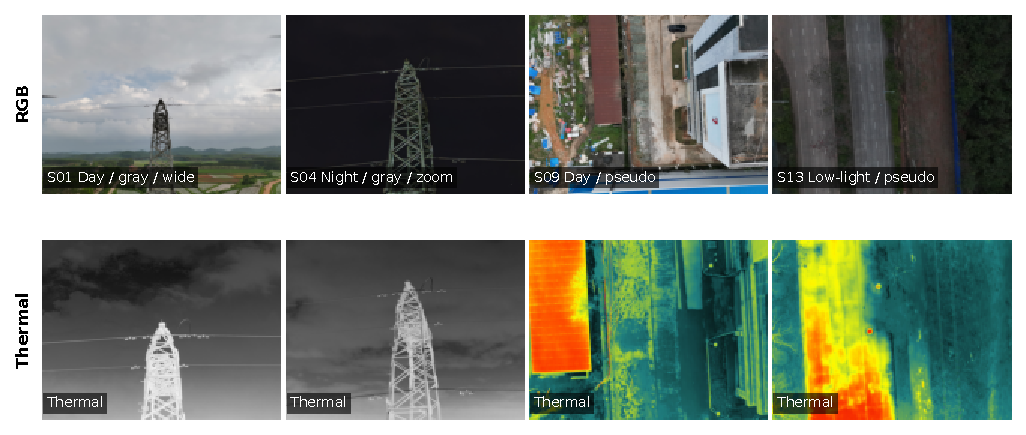
\includegraphics[width=\textwidth]{figures/fig_dataset_examples.pdf}
\caption{UAV-TAlign-12K 的代表性 RGB-红外图像对，覆盖不同光照、热成像渲染和视图条件。}
\label{fig:dataset_examples_zh}
\end{figure}

\subsection{采集与整理}

UAV-TAlign-12K 的采集时间跨度为 2024 年下半年至 2026 年上半年，覆盖中国南部的工业与自然
场景。全部场景均使用同一套 DJI Matrice 350 RTK 平台和 Zenmuse H30T 多传感器载荷采集。
集成载荷自动同步可见光与红外产品，从而保留原生跨传感器几何关系。飞行方式包括悬停和航线式
采集，所用无人机完成实名登记，飞手具有 CAAC 资质，并在允许飞行的空域内执行任务。

发布的数据流保留 H30T 原生采集模式。广角相机静态图像分辨率为 $4032\!\times\!3024$，变焦
相机静态图像为 $3664\!\times\!2748$，热红外图像为 $1280\!\times\!1024$。场景 01 和 02 的
$3840\!\times\!2160$ 静态图像是在 H30T 录像期间触发拍照获得。场景 07 是同步视频抽帧序列，
以每秒 2 帧的频率采样，覆盖无人机环绕输电塔一周的完整过程。灰度场景使用 H30T 的
\emph{White Hot} 设置，伪彩场景使用设备内置的 \emph{Hot Iron} 色板。

数据整理标准在算法评测前冻结，涵盖场景相关性、曝光、对焦和文件完整性。整理后的候选数据集
包含 6,039 对同步图像，完整性审计进一步定义了 6,037 对正式评测划分。筛选过程不使用匹配器
输出、对齐估计或质量分数。

发布准备阶段移除嵌入式元数据并规范化文件名，同时保持图像像素不变。RGB 与红外文件通过共享
的 H30T 采集键关联，按采集时间与序列索引排序，并赋予共同的六位图像对标识。发布过程不进行
缩放、裁剪、旋转、重压缩或图像增强。数据集归广西大学所有，并计划采用知识共享署名 4.0 国际
许可协议发布。

\subsection{数据组织}

每个场景均包含独立的 \texttt{rgb/} 与 \texttt{thermal/} 目录，配对样本具有相同的文件名主干。
正式 manifest 记录场景标识、图像对标识、光照条件、热成像渲染、视图类型和场景标签。一个场景
用于汇集具有共同地点或目标语境及采集条件的帧，可以来自连续序列，也可以来自同一场景定义下的
多次架次。场景 07 是明确记录的单次环绕视频序列。

同一个 manifest 支撑全部成对、场景和条件分析，并把每一项报告结果映射回对应场景与图像对标识。

\subsection{多层评测协议}

基准定义三个互补轨道。轨道 A 独立评测全部 6,037 对图像，衡量成对单应性证据的可用性与支撑度。
轨道 B 将逐帧估计聚合为场景变换，并报告规范定义的高置信场景产品集合。轨道 C 使用固定、可解释
的可靠性分数对场景排序，从而构建覆盖率感知的运行曲线。

三个轨道共同把匹配器输出与可部署场景几何联系起来。成对指标刻画证据生成，场景级指标刻画
多帧共识，运行曲线则反映场景质量变化时产品覆盖率的演变。

\subsection{无标注场景一致性诊断}

该协议采用无标注相对信号进行可扩展的场景一致性分析。所存储的诊断量比较优化后变换与基线初始
变换，并量化跨模态一致性的变化，包括边缘重叠增益、梯度 NCC 增益、梯度一致性改善帧比例、
严重基线相对离群点数量与比例、接受帧支撑、单应性离散度，以及鲁棒剔除比例。

这些信号共同刻画跨模态改善、几何支撑和共识稳定性，并通过统一评测接口支撑规范产品选择、条件
感知分析和可靠性--覆盖率可视化 \cite{ma2021survey,liao2024survey}。

% !TEX root = ../paper_zh.tex

\section{UAV-TAlign 参考框架}

\subsection{问题定义}

UAV-TAlign 用于实例化 UAV-TAlign-12K 的场景级评测轨道。对每个场景，输入是一组配对的无人机
RGB 与红外帧
$S = \{(I_i^R, I_i^T)\}_{i=1}^N$。视点变化、跨分辨率感知、热成像外观差异和光照变化会使
各帧估计具有异质的支撑质量。目标是恢复一个从红外到 RGB 的场景单应性，并刻画其运行置信度。

该定义把配准表述为多帧证据整合问题，而非单对图像选择问题。框架需要把质量不一的逐帧估计
转化为几何稳定且跨模态一致的场景变换。对于一个选定图像对，从红外到 RGB 的证据表示为作用于
齐次图像坐标的单应矩阵 $H_i \in \mathbb{R}^{3 \times 3}$：
\begin{equation}
\tilde{\mathbf{p}}^{R}_{ij} \sim H_i \tilde{\mathbf{p}}^{T}_{ij},
\qquad
H_i = \arg\min_H \sum_{j \in \mathcal{I}_i}
\rho\!\left(\left\|\pi(H\tilde{\mathbf{p}}^{T}_{ij}) -
\mathbf{p}^{R}_{ij}\right\|_2^2\right),
\label{eq:pairwise_homography_zh}
\end{equation}
其中，$\mathcal{I}_i$ 表示鲁棒估计得到的内点集合，$\pi(\cdot)$ 将齐次坐标转换为图像坐标，
$\rho(\cdot)$ 是鲁棒估计损失。场景级问题是在证据集合 $\{H_i\}$ 上估计共识变换
$\bar{H}_S$，并赋予其规范产品状态。

\begin{figure}[t]
\centering
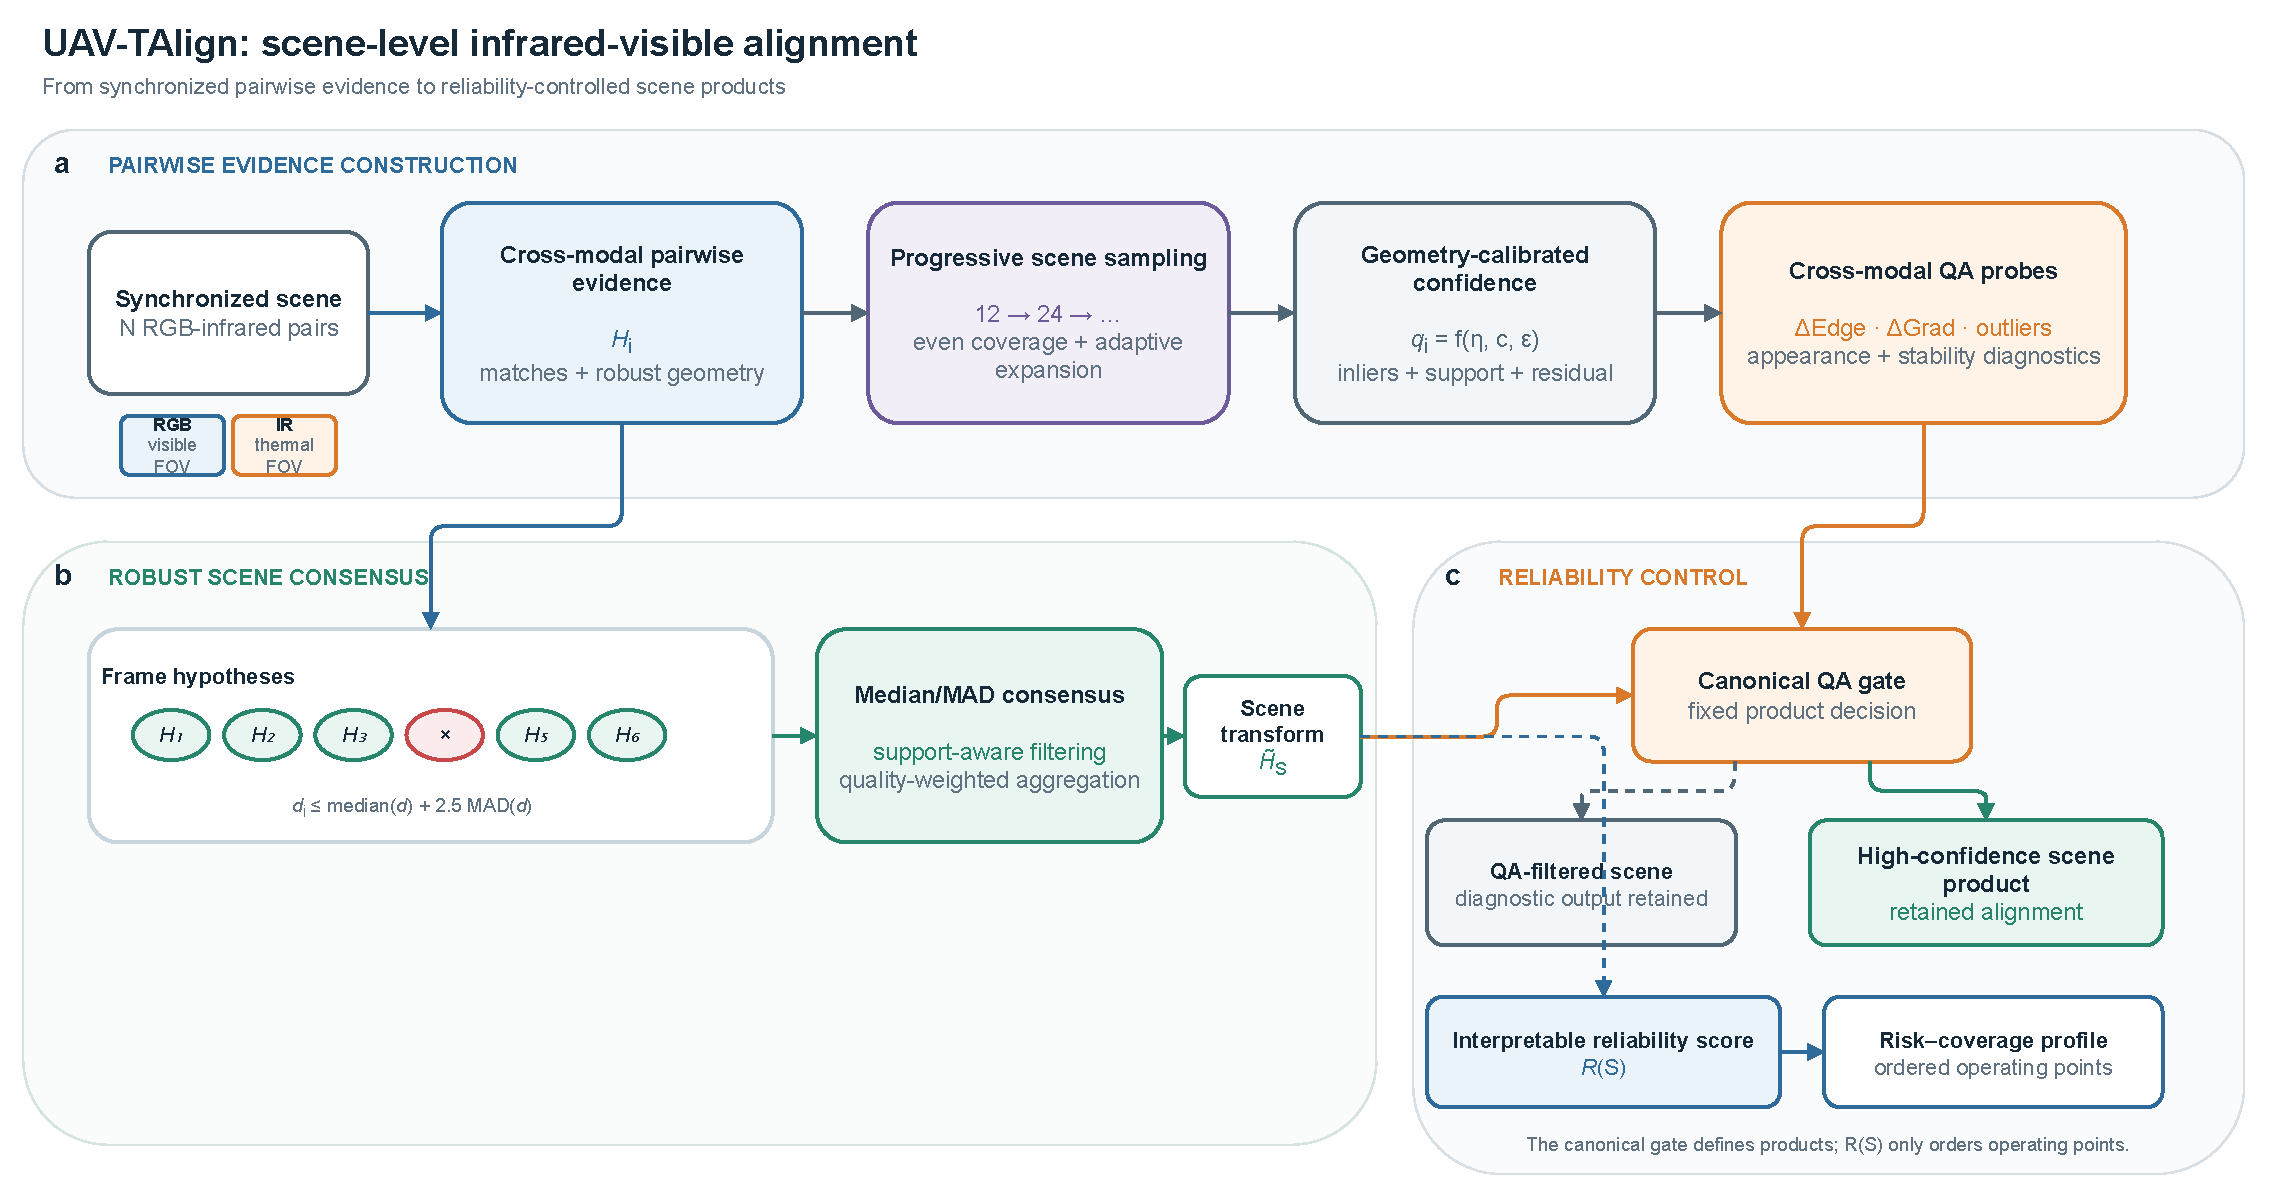
\includegraphics[width=\textwidth]{figures/fig03_scene_framework.pdf}
\caption{UAV-TAlign 场景级对齐框架。（a）同步 RGB-红外图像对依次经过成对单应性生成、渐进式证据
调度、几何校准帧可靠性、鲁棒中位数/MAD 共识和跨模态质量验证；（b）共识支撑外的逐帧假设在固定
规范门控之前被剔除，门控定义高置信产品，可解释分数则独立用于运行覆盖率排序。}
\label{fig:scene_framework_zh}
\end{figure}

\subsection{成对证据生成器}

UAV-TAlign 使用预训练多模态匹配器生成成对证据。参考实现采用 MINIMA 的 RoMa 分支，其余
阶段则可以接收任意兼容匹配器输出的单应性与几何诊断量
\cite{edstedt2024roma,ren2025minima}。

\subsection{渐进式证据调度}

UAV-TAlign 从一个紧凑、均匀分布的帧子集开始，并以确定性阶段逐步扩展支撑集合。调度规模随
场景长度变化，必要时可以覆盖完整序列。当接受支撑、共识稳定性和跨模态质量条件满足时停止扩展；
否则评测下一阶段子集。

在每个阶段内，均匀分布采样提供可复现的时间或索引覆盖。随机选择变体通过独立的多随机种子
敏感性分析进行评测。

\subsection{几何校准帧可靠性}

对于每个选定图像对，匹配器产生跨模态对应关系和逐帧单应性估计。UAV-TAlign 测量匹配数量、
内点支撑、内点率、重投影误差和空间覆盖率。当这些统计量满足几何质量准则时，对应帧进入场景
候选池。该处理遵循标准单应性估计与鲁棒拟合方法
\cite{hartley2004multiple,fischler1981ransac,barath2019magsac,barath2020magsacpp}。

每个接受帧还会获得一个连续质量权重。该权重综合内点率、空间覆盖率、重投影质量、匹配器置信度
以及内点支撑，使具有更强几何依据的单应性在场景聚合中具有更大影响。归一化帧质量权重写为：
\begin{equation}
q_i =
\alpha_r \phi(r_i) +
\alpha_c \phi(c_i) +
\alpha_e \phi(e_i) +
\alpha_m \phi(m_i) +
\alpha_n \phi(n_i),
\qquad
\sum_k \alpha_k = 1,\ \alpha_k \ge 0,
\label{eq:frame_quality_zh}
\end{equation}
其中，$r_i$ 是内点率，$c_i$ 是空间覆盖率，$e_i$ 是重投影质量，$m_i$ 是匹配器置信度，
$n_i$ 是内点支撑，$\phi(\cdot)$ 将各诊断量映射到一致的质量方向。所有 UAV-TAlign-12K
评测均使用固定权重。

\subsection{鲁棒场景共识}

在获得足够的逐帧单应性后，UAV-TAlign 构建鲁棒场景共识。首先将单应性映射到参数空间，以
中位数作为中心参考，并采用中位数绝对偏差（MAD）准则剔除不稳定估计；随后使用上述帧质量分数
对保留单应性进行加权聚合。令 $\mathbf{h}_i$ 表示 $H_i$ 的尺度归一化向量形式，则共识集合为：
\begin{equation}
\begin{aligned}
\mathbf{h}^{\mathrm{med}}_S
&= \operatorname{median}_{j \in \mathcal{A}_S}(\mathbf{h}_j), \\
d_i &= \left\|\mathbf{h}_i - \mathbf{h}^{\mathrm{med}}_S\right\|_2, \\
m_d &= \operatorname{median}_{j \in \mathcal{A}_S}(d_j), \\
s_d &= \operatorname{median}_{j \in \mathcal{A}_S}|d_j-m_d|, \\
\mathcal{C}_S &= \left\{i \in \mathcal{A}_S: d_i \le m_d + 2.5s_d\right\}.
\end{aligned}
\label{eq:consensus_set_zh}
\end{equation}
其中，$\mathcal{A}_S$ 是鲁棒共识前的接受帧集合。场景变换通过质量加权聚合得到：
\begin{equation}
\bar{\mathbf{h}}_S =
\frac{\sum_{i \in \mathcal{C}_S} q_i \mathbf{h}_i}
{\sum_{i \in \mathcal{C}_S} q_i},
\qquad
\bar{H}_S = \operatorname{mat}(\bar{\mathbf{h}}_S).
\label{eq:scene_consensus_zh}
\end{equation}

框架同时记录聚合变换周围的稳定性诊断，包括相对于聚合结果的单应性离散度，以及被鲁棒剔除的
逐帧估计比例。这些诊断量把共识形成过程与最终场景产品决策联系起来。

\subsection{跨模态场景验证}

最后阶段融合几何支撑与跨模态场景一致性。UAV-TAlign 在代表帧上测量优化后变换的边缘重叠增益、
梯度 NCC 增益、改善帧比例和严重相对离群点。同时记录接受帧支撑、平均内点率、平均重投影误差、
空间覆盖率、相对于聚合变换的离散度，以及鲁棒剔除比例。

规范决策采用基线感知验证规则。高置信产品需要同时具备较强的接受帧支撑、稳定的共识几何、
受控的基线相对离群点和改善后的梯度对齐。为绘制运行曲线，使用一个固定、可解释的可靠性分数
汇总同一组诊断量：
\begin{equation}
\begin{aligned}
R(S) ={}&
\beta_a A_S +
\beta_o (1-O_S) +
\beta_j (1-J_S) \\
&+
\beta_e \Delta E_S +
\beta_g \Delta G_S +
\beta_{\gamma} \Gamma_S,
\qquad
\sum_k \beta_k = 1 .
\end{aligned}
\label{eq:reliability_score_zh}
\end{equation}
其中，$A_S$ 是接受帧支撑，$O_S$ 是严重基线相对离群点比例，$J_S$ 是鲁棒共识剔除比例，
$\Delta E_S$ 与 $\Delta G_S$ 分别为边缘和梯度增益代理量，$\Gamma_S$ 汇总几何诊断量。
规范决策要求满足最低接受帧假设数量，并通过两条固定验证路径之一：
\begin{equation}
y_S =
\mathbb{1}\!\left[
N_S \ge N_{\min}
\right]
\mathbb{1}\!\left[L_S \lor W_S\right].
\label{eq:canonical_gate_zh}
\end{equation}
其中，$L_S$ 表示主要边缘/梯度路径，$W_S$ 表示联合接受支撑、共识几何、相对离群点控制和
梯度改善的高模态路径。$R(S)$ 用于可靠性--覆盖率分析中的场景排序，$y_S$ 则定义规范的高置信
对齐产品集合。

图~\ref{fig:consensus_qa_zh} 在一组匹配场景对照上揭示内部证据流：即使接受帧数量相同，引入共识
剔除与跨模态离群点后，仍可得到不同的场景产品决策。

\begin{figure}[t]
\centering
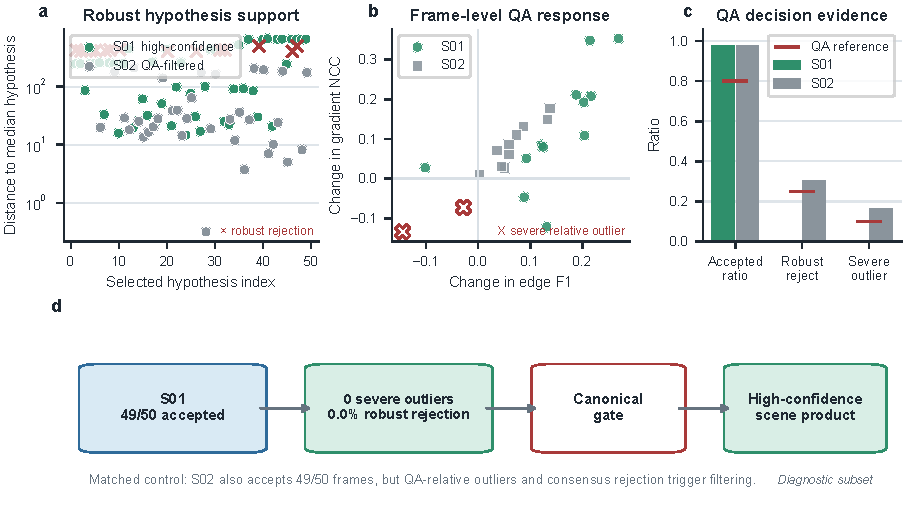
\includegraphics[width=\textwidth]{figures/fig04_consensus_qa.pdf}
\caption{匹配场景对照上的鲁棒共识与跨模态质量验证机制。（a）中位数/MAD 支撑簇确定聚合证据；
（b）逐帧边缘与梯度变化揭示严重相对离群点；（c）接受支撑、鲁棒剔除和离群点控制构成互补决策
证据；（d）固定规范门控将这些信号转换为高置信场景产品。}
\label{fig:consensus_qa_zh}
\end{figure}

% !TEX root = ../paper_zh.tex

\section{实验设置}

\subsection{基线方法}

本文使用公开预训练配置评测七种代表性基线，不针对 UAV-TAlign-12K 进行特定适配。基线覆盖
三个方法类别。SIFT 与 AKAZE 构成经典关键点参考，随后均进行鲁棒单应性估计。RIFT2 通过
Python 实现提供红外-可见光专用经典参考。现代方法包括 Kornia LoFTR、RoMa outdoor、
XoFTR-640 和 raw MINIMA
\cite{sun2021loftr,edstedt2024roma,tuzcuoglu2024xoftr,ren2025minima}。

raw MINIMA 使用 \texttt{minima\_roma} 检查点族和完整 RoMa 分支。RoMa 使用公开 outdoor full
模型，XoFTR 使用 640 分辨率可见光-热红外检查点，LoFTR 使用 Kornia 的公开 outdoor 预训练
模型。统一推理封装在保留各预训练模型的同时，对图像输入输出、模型输出、单应性拟合和结果格式
进行标准化。

\subsection{几何拟合与部署配置}

共享评测器使用 USAC-MAGSAC 将预测对应关系转化为单应性，重投影阈值为 3.0 像素，置信度
为 0.999，最大迭代次数为 10,000，并采用 $4\!\times\!4$ 空间覆盖网格。该公共估计器支持
对集成的成对基线进行一致结果统计。

RIFT2 使用冻结的 resize-aware 配置：\texttt{max\_dim=1200}、\texttt{npt=2000}、
\texttt{patch\_size=64}、Lowe ratio 0.95，并采用 5.0 像素重投影阈值的 USAC-MAGSAC。
LoFTR 使用最长图像边为 1200 的 resize-aware 推理并启用自动混合精度。运行时间和拟合诊断量
均在这些声明的部署配置下报告。

\subsection{协议验证}

本文在冻结的正式输出上开展两项受控实验。五折留帧分析以确定性方式划分接受帧假设，每次留出
一折，重新计算场景共识，并测量其相对完整证据变换的网格位移。受控敏感性实验对每个场景的
3 个代表帧施加平移、旋转和尺度扰动，标称严重度为 2、5、10、20 和 40 像素。实验记录边缘
重叠与梯度 NCC 响应，同时保持规范决策不变。

期刊规模实验在配备 NVIDIA RTX 4090 的工作站上、相互隔离的 Python 环境中完成。主环境采用
Python 3.10、PyTorch 2.0.1、torchvision 0.15.2、CUDA 11.8、OpenCV 4.11.0 和
Kornia 0.6.11。所有实验均使用正式 manifest、固定模型权重或接口、独立输出目录以及只读的
原始数据目录。

% !TEX root = ../paper_zh.tex

\section{实验结果}

\subsection{成对红外-可见光单应性证据}

在 UAV-TAlign-12K 上，成对红外-可见光单应性证据整体具有很高可用性。
表~\ref{tab:pairwise_baselines_zh} 报告完整的 6,037 对正式评测划分。SIFT 和 AKAZE 作为经典
关键点参考，单应性可用率分别达到 87.08\% 和 94.29\%。RIFT2、raw MINIMA 和 RoMa 在每一对
评测图像上均能产生单应性，而 LoFTR 与 XoFTR 的可用率均超过 99\%。这些结果表明，红外专用
方法和现代稠密匹配器均可作为场景级对齐的强证据生成器。

\begin{table}[H]
\caption{UAV-TAlign-12K 上的成对红外-可见光单应性证据。单应性可用率表示鲁棒估计成功的
记录比例，其余列分别刻画声明部署配置下的对应关系支撑、空间范围、拟合残差和运行时间。}
\label{tab:pairwise_baselines_zh}
\centering
\resizebox{\textwidth}{!}{
\begin{tabular}{llrrrrrr}
\toprule
方法 & 类别 & OK / N $\uparrow$ & H (\%) $\uparrow$ & 内点率 $\uparrow$ & 覆盖率 $\uparrow$ & 重投影中位数 $\downarrow$ & 单对时间 (s) $\downarrow$ \\
\midrule
SIFT + RANSAC & 经典关键点 & 5257/6037 & 87.08 & 0.242 & 0.627 & 0.000 & 4.421 \\
AKAZE + RANSAC & 经典关键点 & 5692/6037 & 94.29 & 0.160 & 0.730 & 0.105 & 1.103 \\
RIFT2 (Python, resize-aware) & 红外-可见光经典方法 & 6037/6037 & \textbf{100.00} & 0.086 & 0.354 & 0.121 & 13.980 \\
raw MINIMA & 现代稠密 / 学习型 & 6037/6037 & \textbf{100.00} & 0.319 & 1.000 & 1.773 & 1.346 \\
RoMa outdoor & 现代稠密 / 学习型 & 6037/6037 & \textbf{100.00} & 0.328 & 0.997 & 1.741 & 0.929 \\
Kornia LoFTR outdoor (resize-aware) & 现代稠密 / 学习型 & 5984/6037 & 99.12 & 0.074 & 0.895 & 0.823 & 0.169 \\
XoFTR-640 & 现代稠密 / 学习型 & 5989/6037 & 99.20 & 0.089 & 0.949 & 1.732 & 0.647 \\
\bottomrule
\end{tabular}}
\end{table}

不同方法族呈现互补的证据特性。RIFT2 同时实现完整单应性可用率和较低拟合重投影误差，而 raw
MINIMA 与 RoMa 提供接近完整的空间覆盖。可用性、支撑度和覆盖率共同构成场景级基准轨道的
几何背景。

\begin{figure}[t]
\centering
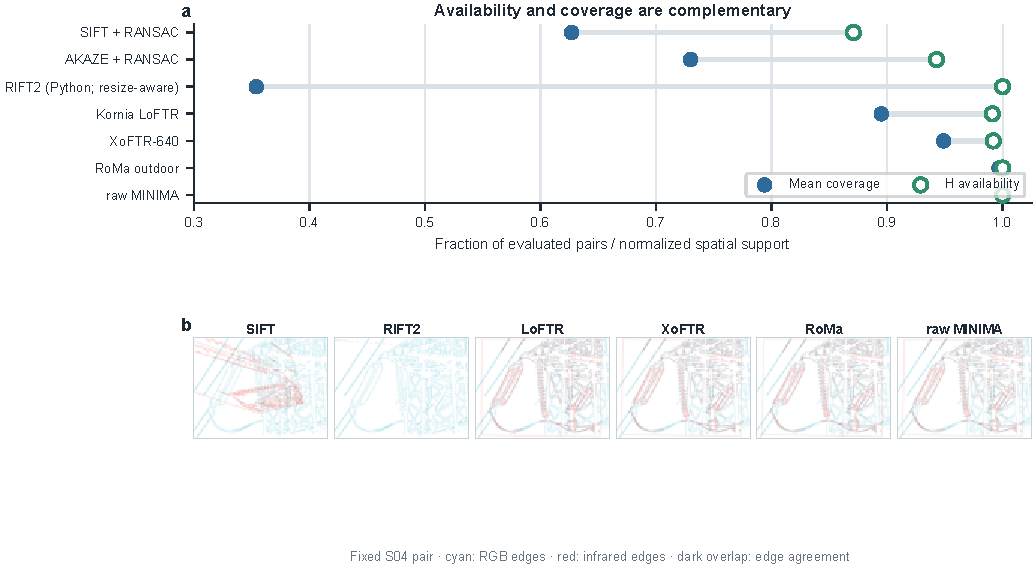
\includegraphics[width=\textwidth]{figures/fig05_pairwise_evidence.pdf}
\caption{不同匹配器家族的成对单应性证据。（a）单应性可用率与平均空间覆盖率从互补角度刻画
6,037 对正式评测划分上的证据完整性；（b）固定图像对的青色/红色边缘叠加，对比统一下游估计器
下代表性经典与学习型匹配器产生的几何支撑。}
\label{fig:pairwise_evidence_zh}
\end{figure}

\subsection{场景级参考结果}

UAV-TAlign 将成对证据转化为全部 15 个场景的变换。在规范运行点，框架识别出 9 个高置信产品，
对应 60.0\% 的场景覆盖率和 74.4\% 的图像对覆盖率。这些产品内部的接受帧支撑为 1491/2304
（64.7\%）。

\begin{table}[H]
\caption{UAV-TAlign 在 UAV-TAlign-12K 上的规范场景级运行点。图像对覆盖率和接受帧支撑均在
9 个高置信场景产品上计算。}
\label{tab:scene_level_main_zh}
\centering
\resizebox{\textwidth}{!}{
\begin{tabular}{llrrrrrr}
\toprule
方法 & 评测单位 & H 可用 $\uparrow$ & 高置信场景 $\uparrow$ & 场景覆盖率 (\%) $\uparrow$ & 图像对覆盖率 (\%) $\uparrow$ & 接受 / 尝试 & 接受率 (\%) $\uparrow$ \\
\midrule
UAV-TAlign & 15 个场景 & 15/15 & 9/15 & 60.0 & 74.4 & 1491/2304 & 64.7 \\
\bottomrule
\end{tabular}}
\end{table}

图~\ref{fig:scene_products_zh} 展示代表性规范对齐产品，覆盖不同光照、红外渲染和视图条件。统一
裁剪区域和边缘一致性视图使跨模态几何改善能够被直接检查。

\begin{figure}[t]
\centering
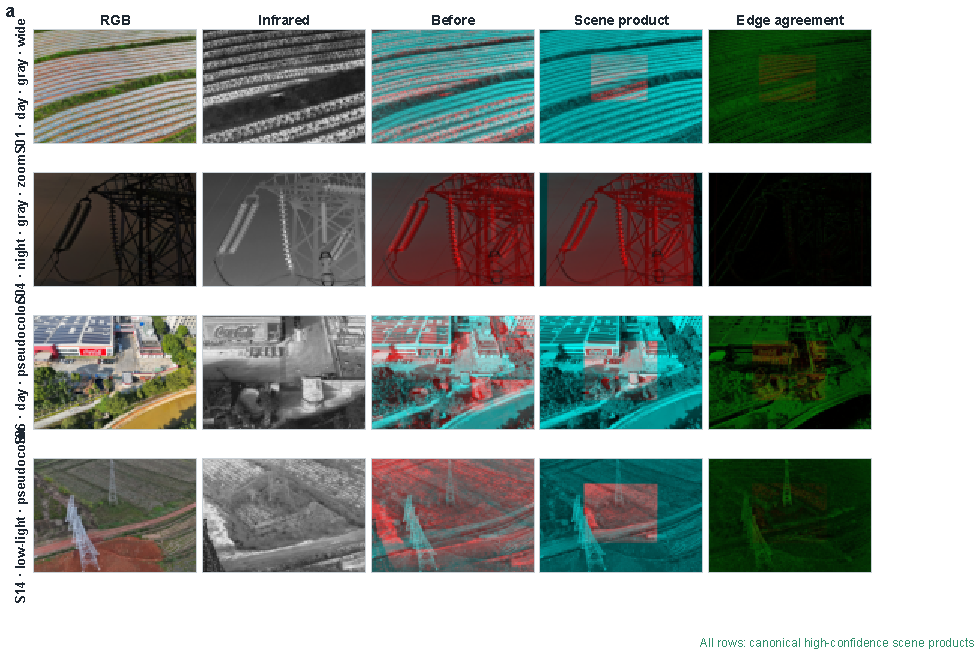
\includegraphics[width=\textwidth]{figures/fig06_scene_products.pdf}
\caption{规范运行点下的代表性 UAV-TAlign 高置信场景产品。各行覆盖白天、夜间与低照度场景，
并包含灰度和设备原生伪彩红外渲染；各列依次展示 RGB 裁剪、红外裁剪、未对齐叠加、场景单应性
叠加和边缘一致性可视化。}
\label{fig:scene_products_zh}
\end{figure}

\subsection{条件感知运行曲线}

不同光照条件呈现不同的场景产品和接受支撑特性。白天采集具有最高的场景覆盖率和接受帧比例；
夜间采集得到 3/5 个高置信产品；低照度采集在 3 个场景中保持 61.3\% 的接受帧比例。这两类互补
测量将可用帧支撑与最终场景产品区分开来。

\begin{table}[H]
\caption{按光照条件统计的运行曲线。接受/尝试表示每种条件下所有场景的汇总帧支撑。}
\label{tab:light_condition_zh}
\centering
\resizebox{\textwidth}{!}{
\begin{tabular}{lrrrrr}
\toprule
条件 & 场景数 & 高置信场景 $\uparrow$ & 场景覆盖率 (\%) $\uparrow$ & 接受 / 尝试 $\uparrow$ & 接受率 (\%) $\uparrow$ \\
\midrule
白天 & 7 & \textbf{5} & \textbf{71.4} & \textbf{1650/2203} & \textbf{74.9} \\
夜间 & 5 & 3 & 60.0 & 361/890 & 40.6 \\
低照度 & 3 & 1 & 33.3 & 462/754 & 61.3 \\
\bottomrule
\end{tabular}}
\end{table}

图~\ref{fig:operating_profile_zh}c,d 将分析扩展到光照、红外渲染与视图类型，同时报告场景保留率
和接受帧支撑。

\subsection{可靠性控制的场景选择}

匹配场景对照说明了为何成对支撑不能单独决定最终产品集合。图~\ref{fig:reliability_selection_zh}
在相同输出视图下比较广角/变焦和夜间对照，并将全部 15 个场景投影到接受支撑与严重离群点空间。
规范产品集中在低离群区域，而接受帧比例横跨保留场景与质量过滤场景。

\begin{figure}[t]
\centering
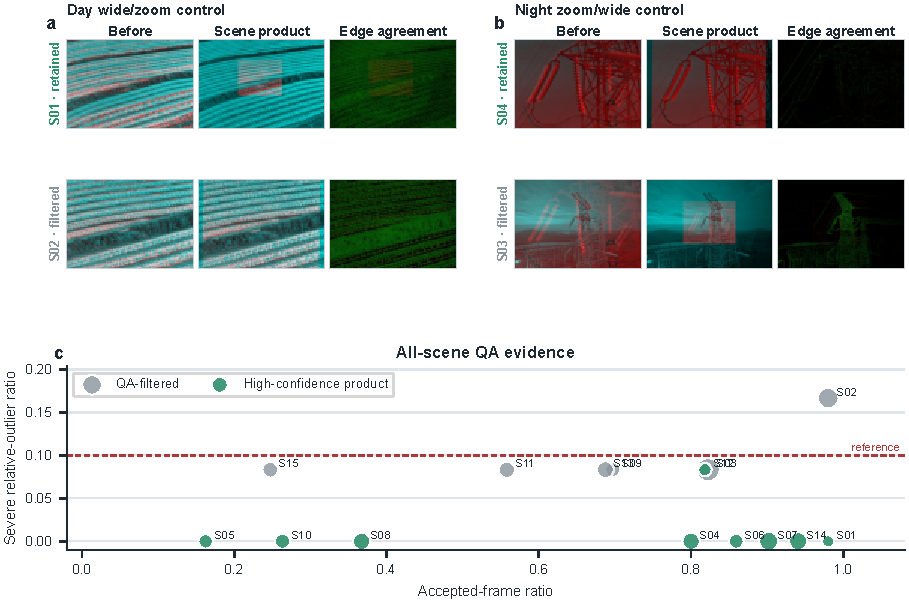
\includegraphics[width=\textwidth]{figures/fig07_reliability_selection.pdf}
\caption{匹配场景条件下的可靠性控制选择。（a,b）广角/变焦与夜间成对对照表明，较强成对支撑仍可
对应不同的规范场景结果；（c）在全部 15 个场景中，规范产品集中于较低严重离群点区域，而接受帧
比例不能单独决定保留结果。标记大小表示鲁棒剔除比例。}
\label{fig:reliability_selection_zh}
\end{figure}

\subsection{可靠性--覆盖率运行曲线}

固定的跨模态验证规则定义规范产品集合，可解释分数则对场景排序以形成连续的可靠性--覆盖率扫描。
图~\ref{fig:operating_profile_zh} 绘制基于分数排序的曲线，并叠加固定的规范运行点。

\begin{figure}[t]
\centering
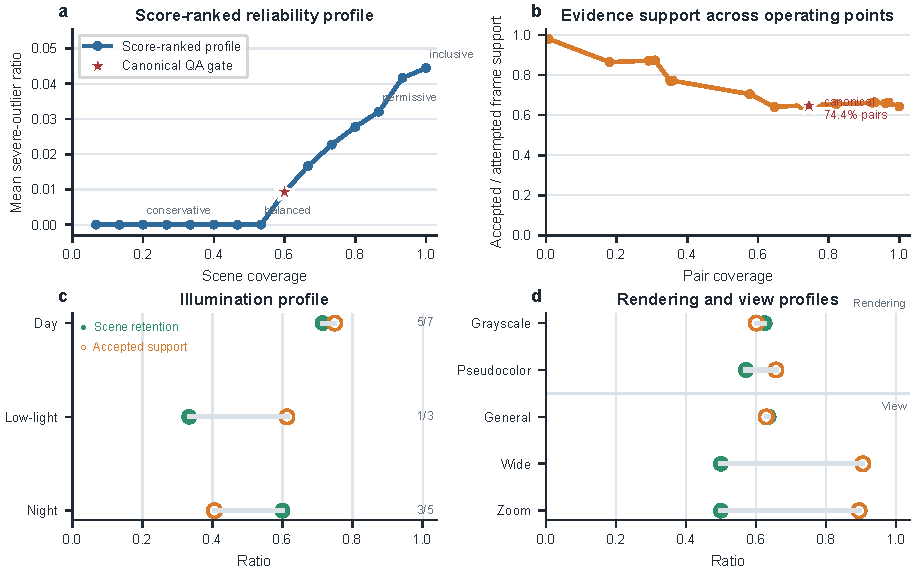
\includegraphics[width=\textwidth]{figures/fig08_operating_profile.pdf}
\caption{UAV-TAlign-12K 上的可靠性--覆盖率运行曲线。（a）基于分数排序的曲线刻画场景覆盖率提高
时的平均严重离群点比例，星号表示独立的规范 QA 运行点，而非分数排序的前九场景；（b）图像对
覆盖率和接受帧支撑给出相应证据范围；（c,d）条件感知曲线汇总光照、红外渲染与视图类型。}
\label{fig:operating_profile_zh}
\end{figure}

在规范运行点，UAV-TAlign 识别出 9 个高置信产品，覆盖 60.0\% 的场景和 74.4\% 的评测图像对，
平均严重离群点比例为 0.009。基于分数排序的曲线提供了从高置信运行到更广覆盖范围的平滑过渡。
图~\ref{fig:operating_profile_zh} 中的规范点对应 9/15 个场景、60.0\% 场景覆盖率和 74.4\% 图像对
覆盖率。

\subsection{场景诊断的受控验证}

场景诊断量在独立重采样和受控几何扰动下表现出一致响应。五折留帧分析覆盖全部 15 个场景和
75 次共识重计算。每折留出约五分之一的接受帧假设时，相对完整证据共识的位移中位数为 1.39
像素，平均值为 2.26 像素。

扰动实验覆盖 45 个代表帧和 675 次受控试验。在每一种扰动类型中，随严重度提高，联合边缘/梯度
质量信号均单调下降。在最大扰动严重度下，平移、旋转和尺度扰动引起的平均联合分数变化分别为
$-0.074$、$-0.031$ 和 $-0.025$，相应退化比例为 84.4\%、80.0\% 和 73.3\%。
表~\ref{tab:protocol_validation_zh} 汇总了这些独立证据。
图~\ref{fig:validation_attribution_zh}a,b 进一步展示逐场景重采样响应和随扰动强度变化的质量趋势。

\begin{table}[H]
\caption{场景共识稳定性与跨模态质量敏感性的受控验证。合成退化比例和联合分数变化均在最大测试
严重度下报告。}
\label{tab:protocol_validation_zh}
\centering
\resizebox{0.92\textwidth}{!}{
\begin{tabular}{llrr}
\toprule
验证方式 & 范围 & 主要响应 & 退化试验 (\%) \\
\midrule
留帧共识 & 15 个场景 / 75 折 & 1.39 px 场景中位漂移 & -- \\
合成平移 & 45 帧 / 225 次试验 & $\Delta$Joint $=-0.074$ & 84.4 \\
合成旋转 & 45 帧 / 225 次试验 & $\Delta$Joint $=-0.031$ & 80.0 \\
合成尺度 & 45 帧 / 225 次试验 & $\Delta$Joint $=-0.025$ & 73.3 \\
\bottomrule
\end{tabular}}
\end{table}

\subsection{累加式消融实验}

固定 8 场景消融用于分离鲁棒共识和跨模态验证的作用。鲁棒共识将平均边缘增益从 0.124 提高到
0.146，将梯度 NCC 增益从 0.126 提高到 0.149；同时，严重离群点比例从 0.104 降至 0.042，
变换离散度从 151.2 像素降至 52.5 像素。跨模态验证进一步把阶段输出映射为规范产品决策。

\begin{table}[H]
\caption{固定 8 场景 UAV-TAlign-1K-Lite 子集上的累加式消融。}
\label{tab:ablation_main_zh}
\centering
\resizebox{\textwidth}{!}{
\begin{tabular}{lcccrrrrr}
\toprule
变体 & 选择 & 共识 & 验证 & 阶段通过/N $\uparrow$ & $\Delta$Edge $\uparrow$ & $\Delta$Grad $\uparrow$ & Severe $\downarrow$ & Disp. (px) $\downarrow$ \\
\midrule
仅成对证据 & even & \xmark & \xmark & 8/8 & 0.124 & 0.126 & 0.104 & 151.2 \\
+ 鲁棒场景共识 & even & \cmark & \xmark & 8/8 & 0.146 & 0.149 & 0.042 & 52.5 \\
+ 跨模态验证 & even & \cmark & \cmark & 5/8 & 0.146 & 0.148 & 0.042 & 57.7 \\
\bottomrule
\end{tabular}}
\end{table}

图~\ref{fig:validation_attribution_zh}c,d 将累加式模块效应与多随机种子选择分析联系起来：鲁棒共识
贡献最大的诊断增益，而确定性调度提供稳定的参考运行策略。

\begin{figure}[t]
\centering
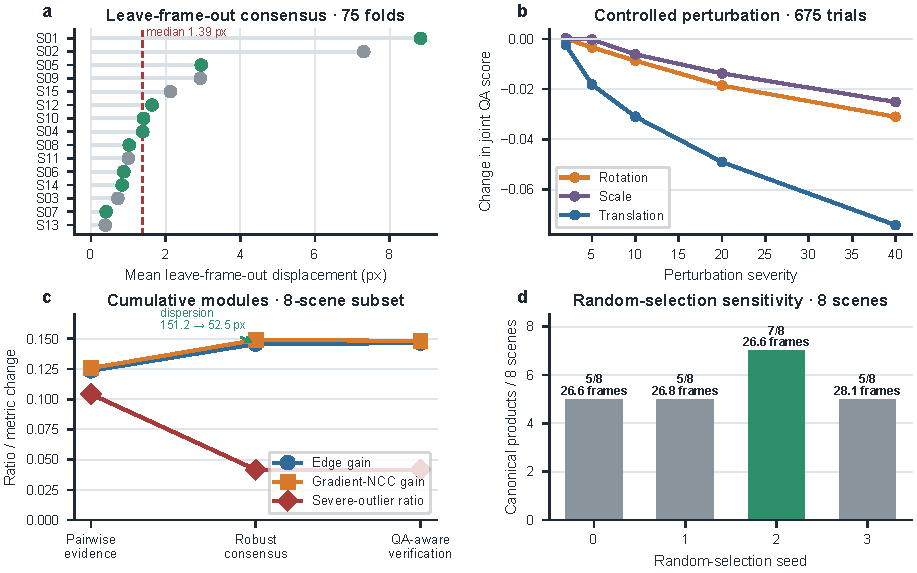
\includegraphics[width=\textwidth]{figures/fig09_validation_attribution.pdf}
\caption{受控验证与模块归因。（a）全部 15 个场景上的五折留帧共识；（b）随平移、旋转与尺度扰动
增强而变化的联合边缘/梯度质量；（c）固定八场景诊断子集上的累加式模块效应；（d）同一子集上
不同随机种子的选择敏感性。}
\label{fig:validation_attribution_zh}
\end{figure}

在不同随机选择种子下，同一固定子集得到 5/8 至 7/8 个场景产品，而平均接受帧支撑保持相对稳定。
该结果确认确定性均匀选择是一种可复现的运行策略，并将随机种子敏感性定位于少量接近阈值的场景。

% !TEX root = ../paper_zh.tex

\section{讨论}

\subsection{从成对证据到场景级几何}

UAV-TAlign-12K 揭示了无人机红外-可见光对齐问题中的一个阶段转变。红外专用方法和现代匹配器
在正式划分的几乎每一对图像上均能生成单应性，从而提供丰富的几何证据。然而，这些证据在空间
支撑、跨模态一致性，以及与同一场景其他帧的一致程度上仍有差异。因此，场景共识是一个独立的
对齐阶段：它将异质逐帧估计转化为可作为统一几何产品使用的场景变换。

消融结果表明，鲁棒共识是贡献最显著的模块。相较仅使用成对证据，共识在提高边缘与梯度一致性的
同时，大幅降低严重离群点比例和变换离散度。跨模态验证随后把稳定几何映射为规范高置信产品集合。
这一组合设计将局部对应关系证据与无人机巡检和多模态感知所需的场景级输出联系起来。

\subsection{覆盖率感知的运行分析}

可靠性--覆盖率曲线为固定阈值评测增加了运行维度。规范运行点提供 9 个高置信产品，并覆盖
74.4\% 的评测图像对；基于分数的扫描则展示更广泛的覆盖区间。应用系统可以据此按照自身质量
要求选择场景产品覆盖率，而无需改变成对匹配器或共识估计器。

两项受控分析支撑了曲线中采用的排序信号。留帧重计算相对完整证据共识仅产生 1.39 像素的漂移
中位数；平移、旋转和尺度扰动也使联合边缘/梯度信号单调下降。这些结果共同把场景诊断量与证据
稳定性和已知几何退化联系起来。

\subsection{基准扩展性}

该基准通过基于 manifest 的接口分离成对对应关系、场景聚合和跨模态验证。未来匹配器可以作为
证据生成器进行比较，也可以在不改变真实采集划分的前提下研究替代共识估计器和运行策略。同一
组织方式还支持扩展到更多场景类别、采集几何、传感器载荷和下游红外感知任务。

确定性证据调度为这一共享接口提供稳定默认策略。多随机种子实验表明，随机选择会改变少量接近
阈值场景的产品状态，但接受帧支撑总体保持稳定。因此，证据调度主要承担可复现性作用，而鲁棒
共识与跨模态验证构成场景产品生成的核心部分。

% !TEX root = ../paper_zh.tex

\section{结论}

本文提出 UAV-TAlign-12K，一个基准规模的无人机红外-可见光对齐资源。它包含 6,039 对同步
图像、经过完整性检查的 6,037 对正式评测划分，以及覆盖成对证据、场景共识和可靠性--覆盖率
分析的多层协议。七种代表性基线表明，红外专用方法和现代匹配器已经能够在真实采集跨视场条件下
提供高可用性的成对单应性。

UAV-TAlign 将这些证据转化为 15 个场景变换。框架结合渐进式调度、几何校准帧加权、鲁棒共识
和跨模态验证，并在规范运行点识别出 9 个高置信产品，覆盖 74.4\% 的评测图像对。留帧重采样和
受控扰动进一步支撑了场景诊断量的稳定性及其对几何变化的敏感性。这些结果表明，场景级证据整合
与置信度感知运行分析是跨视场无人机红外-可见光对齐中的核心评测维度。

\section*{数据可用性}

UAV-TAlign-12K、正式评测 manifest、元数据、完整性报告和评测脚本均已为公开发布做好准备。
正式评测划分包含 6,039 对无人机红外-可见光对齐数据中的 6,037 对完整性检查 RGB-红外图像。
数据集归广西大学所有，将采用知识共享署名 4.0 国际许可协议发布；代码与评测材料将通过公共
仓库提供。同行评审期间可提供审稿访问权限，正式 manifest 哈希将用于保证评测可复现性。


\bibliographystyle{elsarticle-num}
\bibliography{references}

\end{document}
